\section{Port sequences}
\label{s:PortSequences}

During the analysis of the port sequence, where each scanning type was compared between the respective timing templates, there were some interesting findings.

First, the IP ID field was plotted together with the source port for each conducted scan.
Figure \ref{fig:IPIDSrcPort} shows diagrams of various types of scans with various timing templates.
Common for 5 of these scanning types is that the scan uses the same source port for all sent packets, as the figure shows, though the sneaky and paranoid scans must be elaborated further.
The TCP SYN scan could be viewed as artwork, illustrated in figure \ref{fig:TCPSynIPIDSrc}, which shows colors all over the specter which means it uses a different source port for each sent packet.
Figure \ref{fig:XmasInsIPIDSrc}, \ref{fig:NullNormIPIDSrc} and \ref{fig:SvcPolIPIDSrc} shows each 10 lines in each of the figures, which means the same source port are applied to each scan conducted.
The same applies to the sneaky and paranoid scan shown in figure \ref{fig:FinSneIPIDSrc} and \ref{fig:PinParIPIDSrc}, though in a limited way since these two-timing templates bring a different pattern into the diagram. The diagram still shows ten solid lines, but it also shows source ports that are close to the solid line, which makes the given source ports not only 10 but more.



\begin{figure}[!ht]%
    \centering
    \subfloat[xmas insane\label{fig:XmasInsIPIDSrc}]{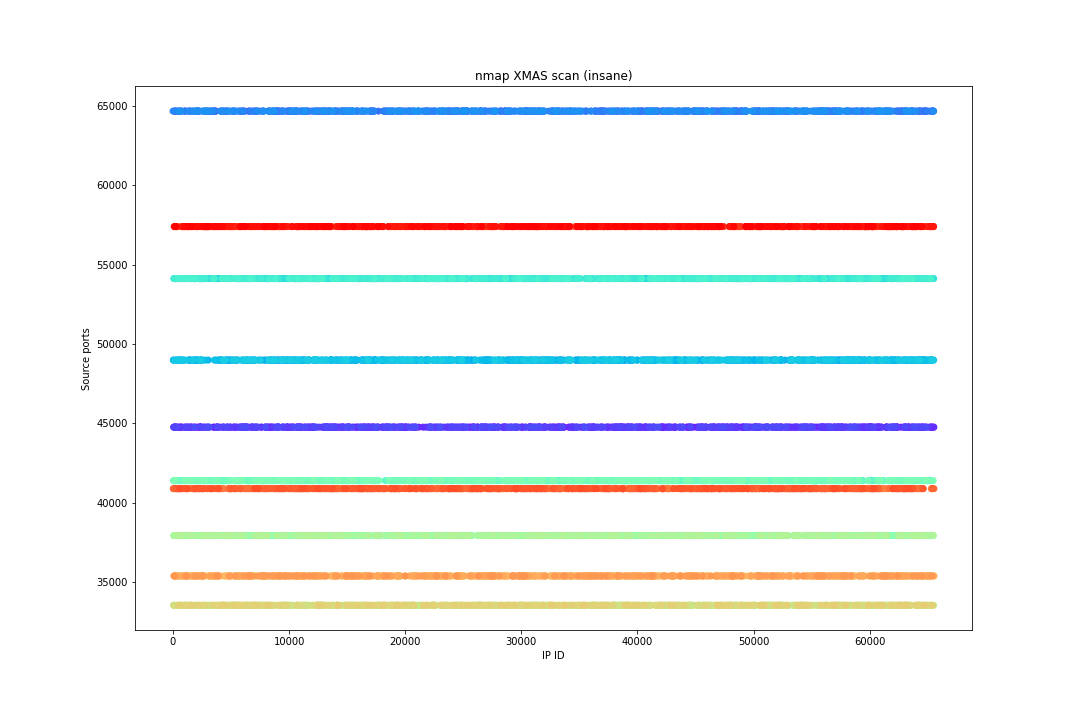
\includegraphics[width=8.2cm]{images/analysis/xmasscan/insane/IPIDSrcPort.png} }
    \subfloat[TCP SYN aggressive\label{fig:TCPSynIPIDSrc}]{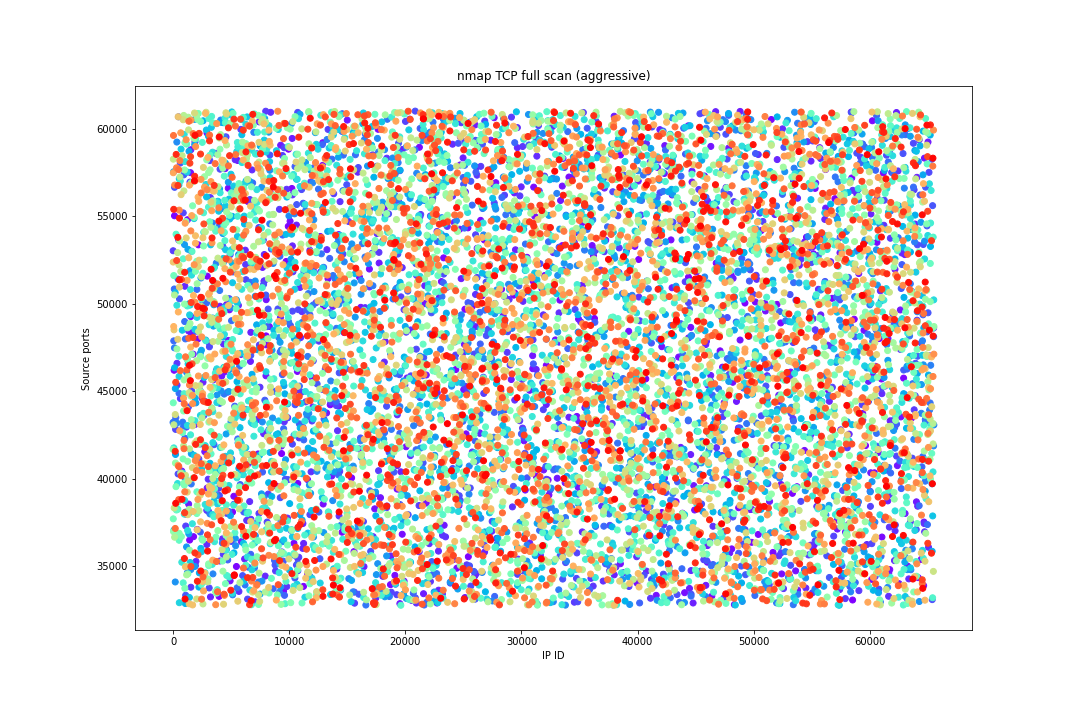
\includegraphics[width=8.2cm]{images/analysis/tcpsynscan/aggressive/IPIDSrcPort.png} }\\
    \subfloat[null scan normal\label{fig:NullNormIPIDSrc}]{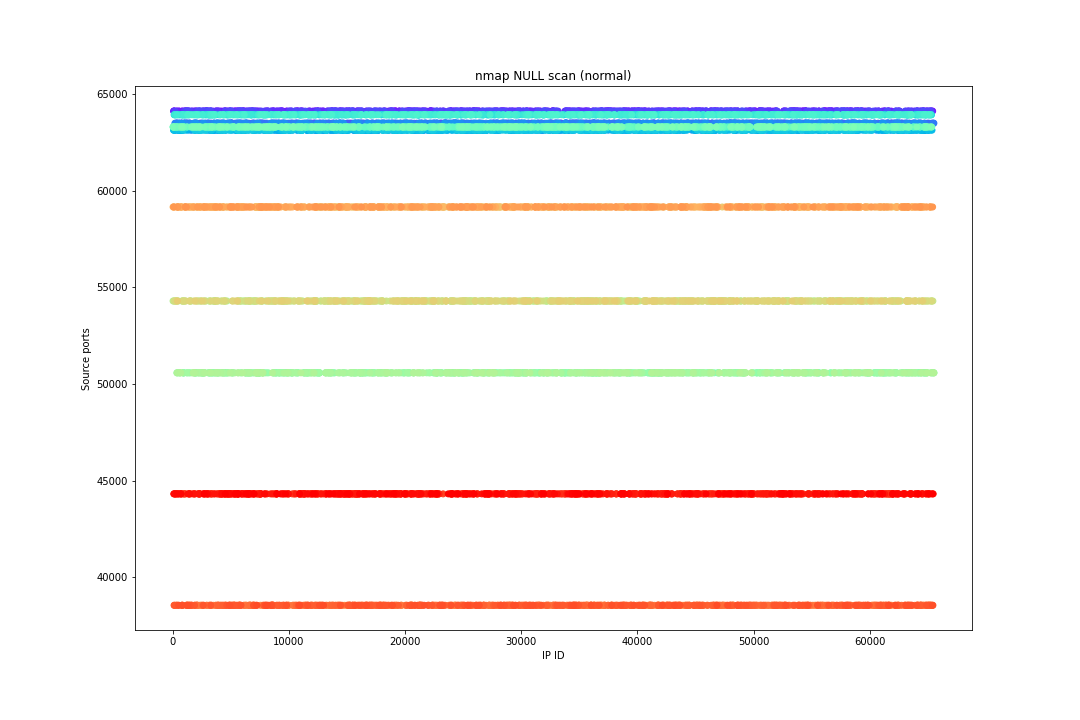
\includegraphics[width=8.2cm]{images/analysis/nullscan/normal/IPIDSrcPort.png} }
    \subfloat[service discovery polite\label{fig:SvcPolIPIDSrc}]{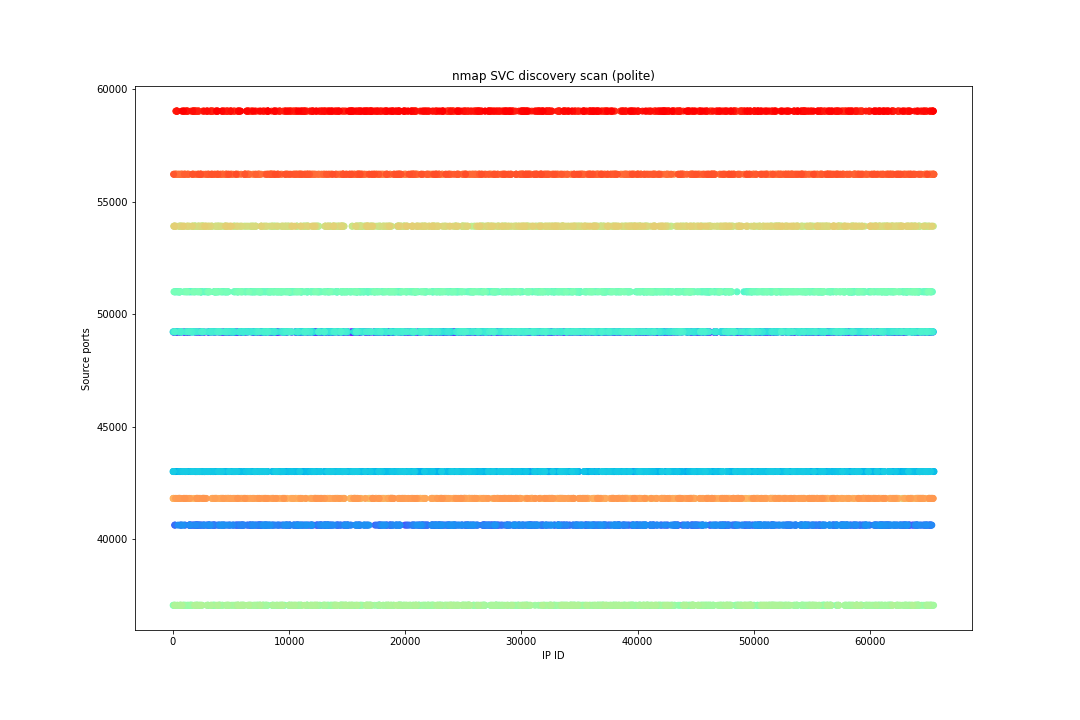
\includegraphics[width=8.2cm]{images/analysis/svcscan/polite/IPIDSrcPort.png} } \\
    \subfloat[fin scan sneaky\label{fig:FinSneIPIDSrc}]{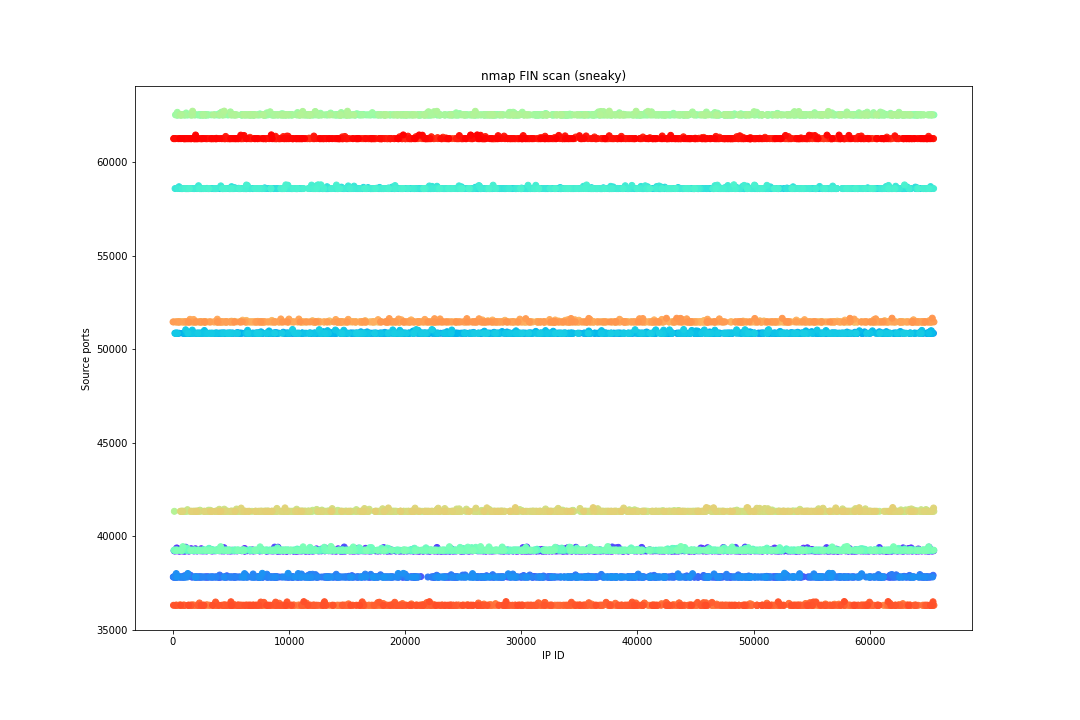
\includegraphics[width=8.2cm]{images/analysis/finscan/sneaky/IPIDSrcPort.png} }
    \subfloat[ping scan paranoid\label{fig:PinParIPIDSrc}]{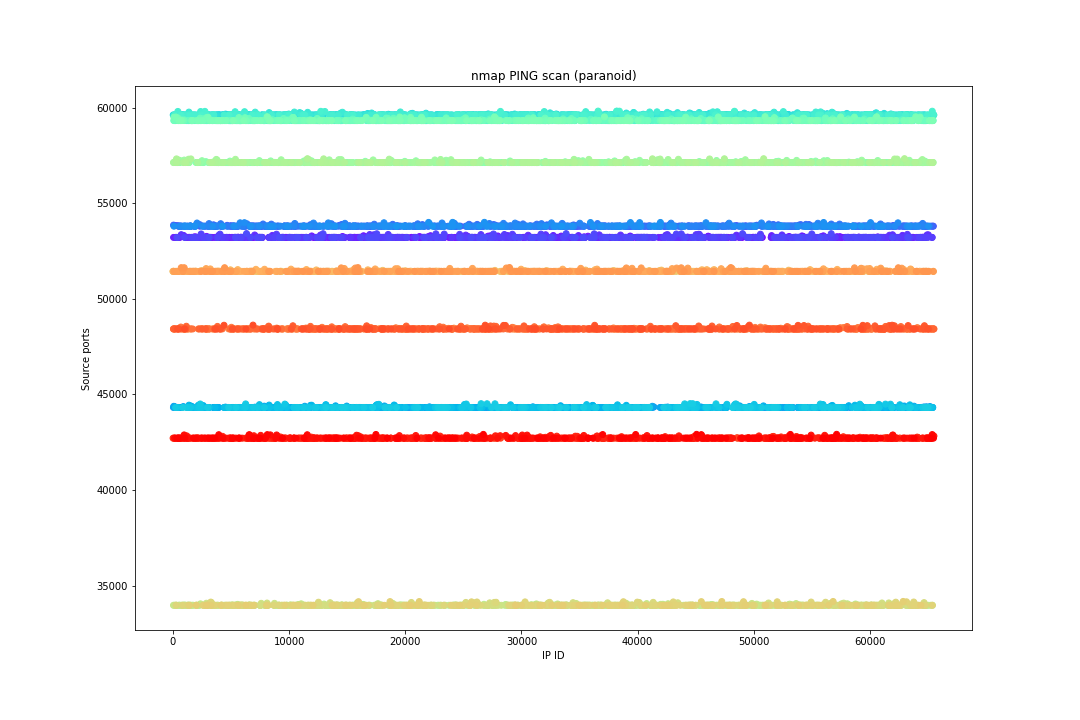
\includegraphics[width=8.2cm]{images/analysis/pingscan/paranoid/IPIDSrcPort.png} }
    \caption{Diagram of IP ID and source ports with various scan types and timing templates}%
    \label{fig:IPIDSrcPort}%
\end{figure}

Within the Jupyter notebook a simple line of code could be applied to further investigate why it appears "feathers" on the sneaky and paranoid scan, shown in listing \ref{lst:FeatherInvestigation}.

\begin{listing}[!ht]
\caption{Print unique source ports and length}
\label{lst:FeatherInvestigation}
\begin{minted}{python}
set(orders_port['sport'])
len(set(orders_port['sport']))
\end{minted}
\end{listing}

This line of code extracts each unique source port during the ten scans of the chosen scanning type with the corresponding timing template.
Further investigation on the paranoid ping scan shown in figure \ref{fig:PinParIPIDSrc} shows 1000 unique source ports for this scan, while the sneaky fin scan in figure \ref{fig:FinSneIPIDSrc} uses 915 unique source ports.
Worth investigating is the aggressive TCP SYN scan as well, as the figure \ref{fig:TCPSynIPIDSrc} shows dots all over the diagram.
By applying the same code to this scan in Jupyter, the number of unique source ports used for this scan is 7122 ports.
Since these scans in figure \ref{fig:IPIDSrcPort} each are a different type and different timing templates, investigating the usage of unique source ports is conducted and shown in table \ref{tbl:UniqueSourcePorts}.
This proves that all of the chosen scanning types except the TCP SYN scan have one dedicated unique source port for each conducted scan for the insane, aggressive, normal, and polite timing template.


\begin{table}[htbp]
\caption{Number of unique source ports}
\begin{center}

\begin{tabular}{|r|r|r|r|r|r|r|}
\hline
scan type & insane & aggressive & normal & polite & sneaky & paranoid\\
\hline
xmas scan & 10 & 10 & 10 & 10 & 1000 & 999\\
\hline
fin scan & 10 & 10 & 10 & 10 & 915 & 910\\
\hline
null scan & 10 & 10 & 10 & 10 & 1000 & 975\\
\hline
ping scan & 10 & 10 & 10 & 10 & 1000 & 1000\\
\hline
tcp full scan & 7108 & 7122 & 7116 & 7144 & 7743 & 7664\\
\hline
svc & 10 & 10 & 10 & 10 & 967 & 998\\
\hline
\end{tabular}
\label{tbl:UniqueSourcePorts}
\end{center}
\end{table}

To further examine the retrieved source ports, the command in listing \ref{lst:SourcePrtInvestigation} can be applied to the Jupyter notebook to list up the top 30 source ports with a count of how many times they were used.

\begin{listing}[!ht]
\caption{Investigating top 30 unique source ports}
\label{lst:SourcePrtInvestigation}
\begin{minted}{python}
orders_port['sport'].value_counts()[:30]
\end{minted}
\end{listing}

On all of the conducted paranoid and sneaky scans, except for the TCP SYN scan, the top 10 source ports are counted either 1000 or 1001 times. The 1001 count appears four times among all the mentioned scans, while 1000 is the regular count seen. This could be shown in the figure \ref{fig:JupyterSvcSrcPort} where we see the top 10 has a count of 1000 or 1001.

\begin{figure}[ht]%
    \centering
    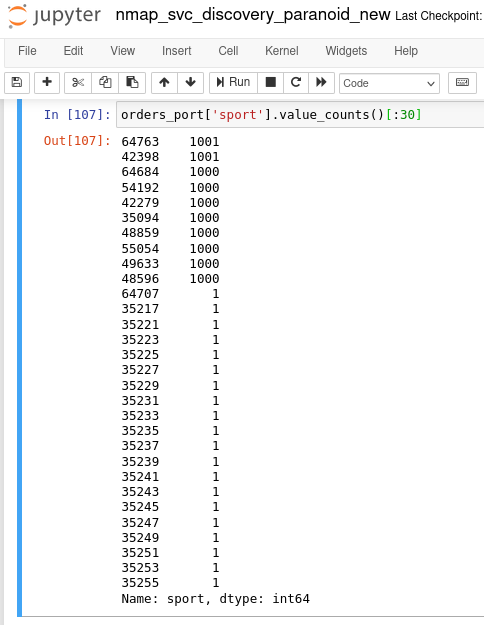
\includegraphics[scale=0.35]{images/analysis/svcscan/JupyterSvcSrcUniquePorts.png}
    \caption{Jupyter notebook top 30 source ports used in Service Discovery scan}%
    \label{fig:JupyterSvcSrcPort}%
\end{figure}



By comparing the various types of scans, each represented with its own timing template, there are definitely similarities between the conducted scans. The port sequence scatter plot in figure \ref{fig:DstPortSequenceMisc} clearly outlines this.
Within the figure, each color symbolizes a unique source port number,
The highest amount of destination ports reached is located close to and below port 1000.
This similarity is clear evidence that Nmap focuses on ports around this port range.
Other interesting characteristics of this figure are the line right above port 30000 and the line right below port 50000.

\vfill
\clearpage

\newpage
\vfill
\begin{figure}[!ht]%
    \centering
    \subfloat[fin scan insane\label{fig:FinInsDstPck}]{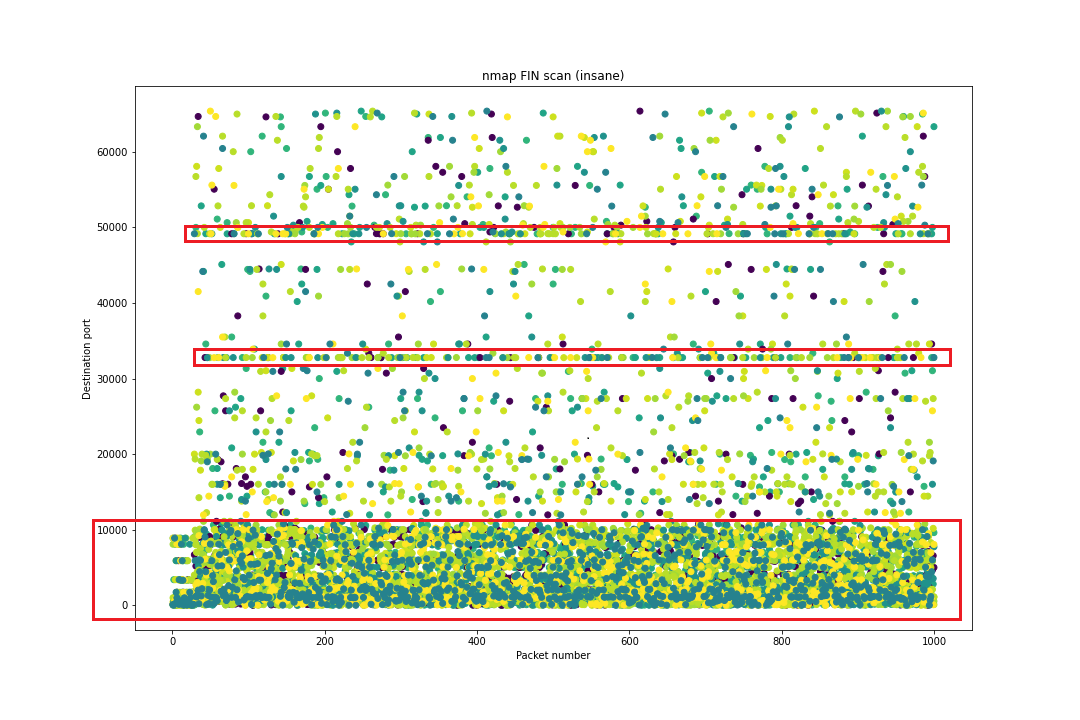
\includegraphics[width=8.2cm]{images/analysis/finscan/insane/DstPacketNrMarked.png} }
    \subfloat[ping scan aggressive\label{fig:PngAgrDstPck}]{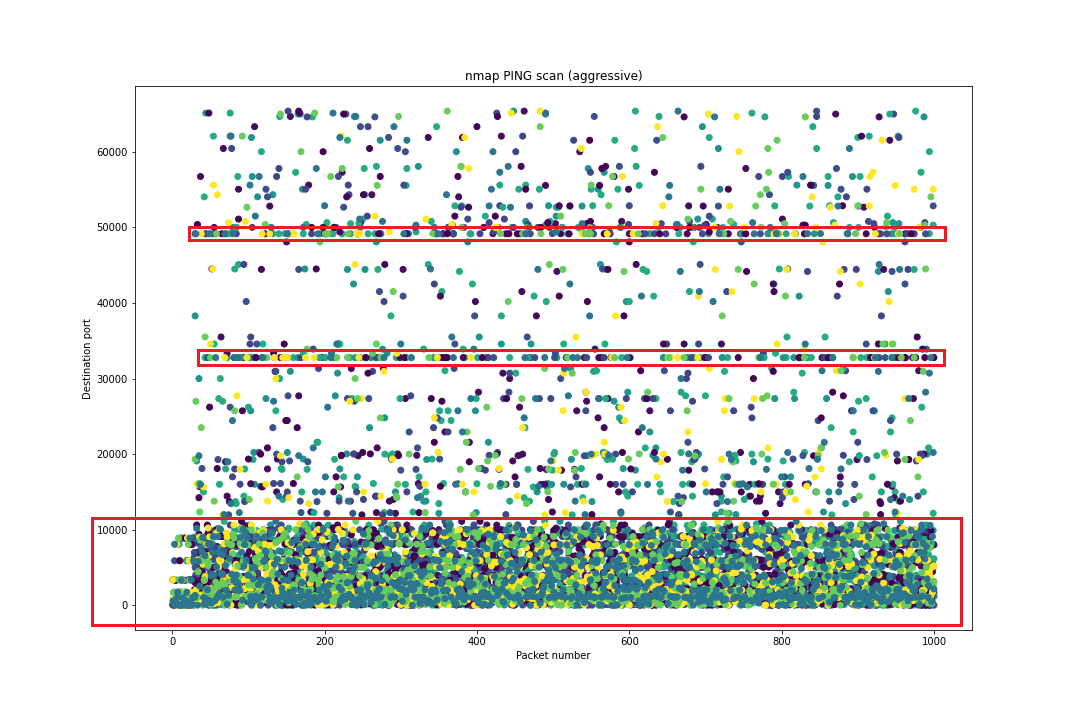
\includegraphics[width=8.2cm]{images/analysis/pingscan/aggressive/DstPacketNrMarked.png} } \\
    \subfloat[service discovery normal\label{fig:SvcNorDstPck}]{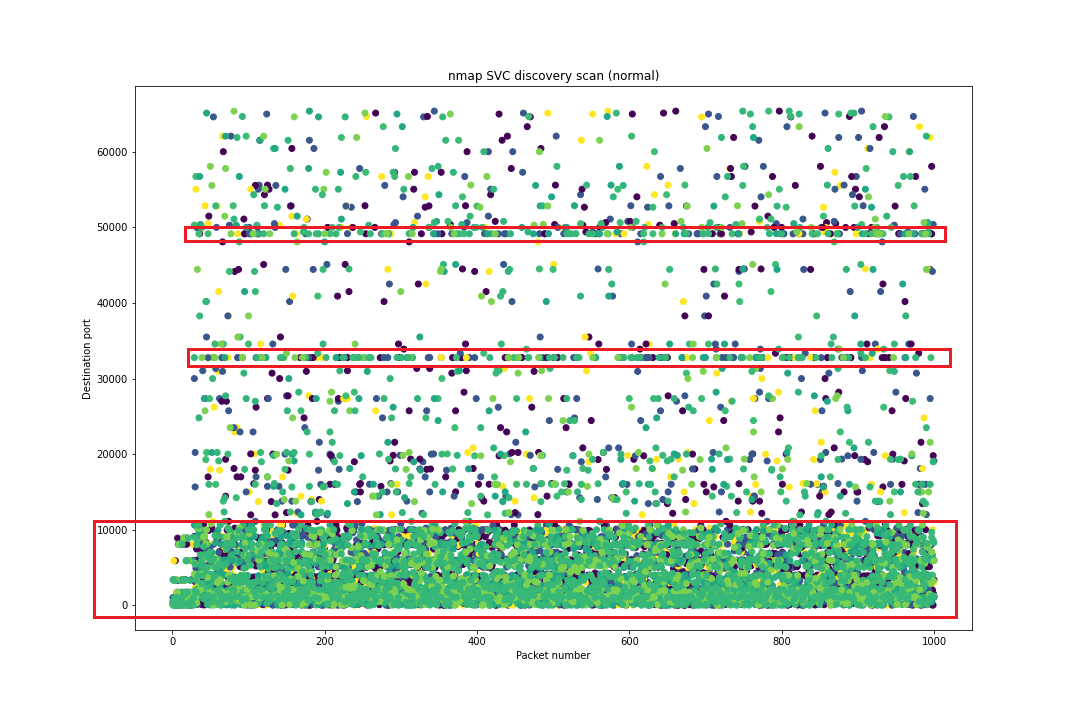
\includegraphics[width=8.2cm]{images/analysis/svcscan/normal/DstPacketNrMarked.png} }
    \subfloat[null scan polite\label{fig:NullPolDstPck}]{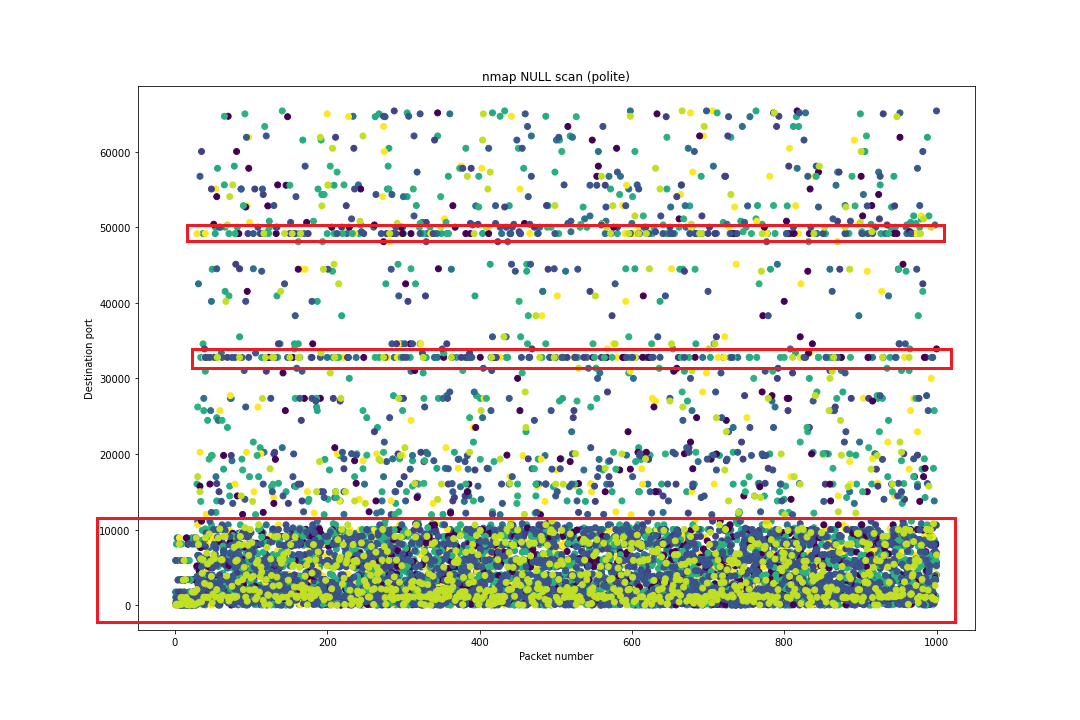
\includegraphics[width=8.2cm]{images/analysis/nullscan/polite/DstPacketNrMarked.png} } \\
    \subfloat[xmas scan sneaky\label{fig:XmasSneDstPck}]{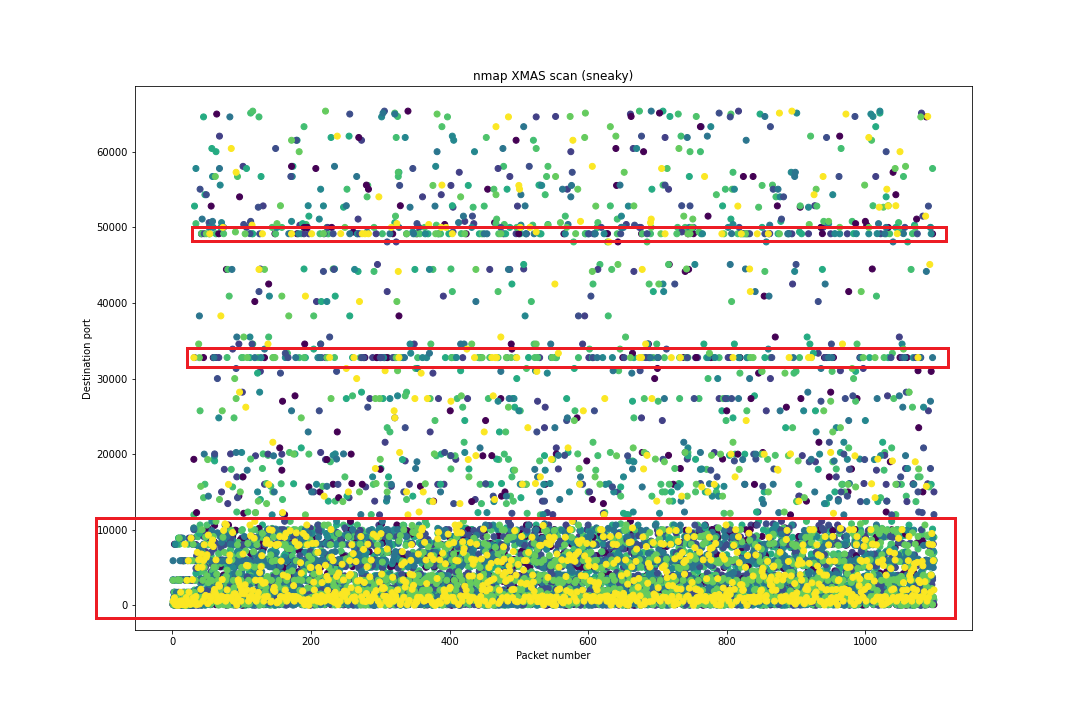
\includegraphics[width=8.2cm]{images/analysis/xmasscan/sneaky/DstPacketNrMarked.png} }
    \subfloat[TCP SYN paranoid\label{fig:TcpParDstPck}]{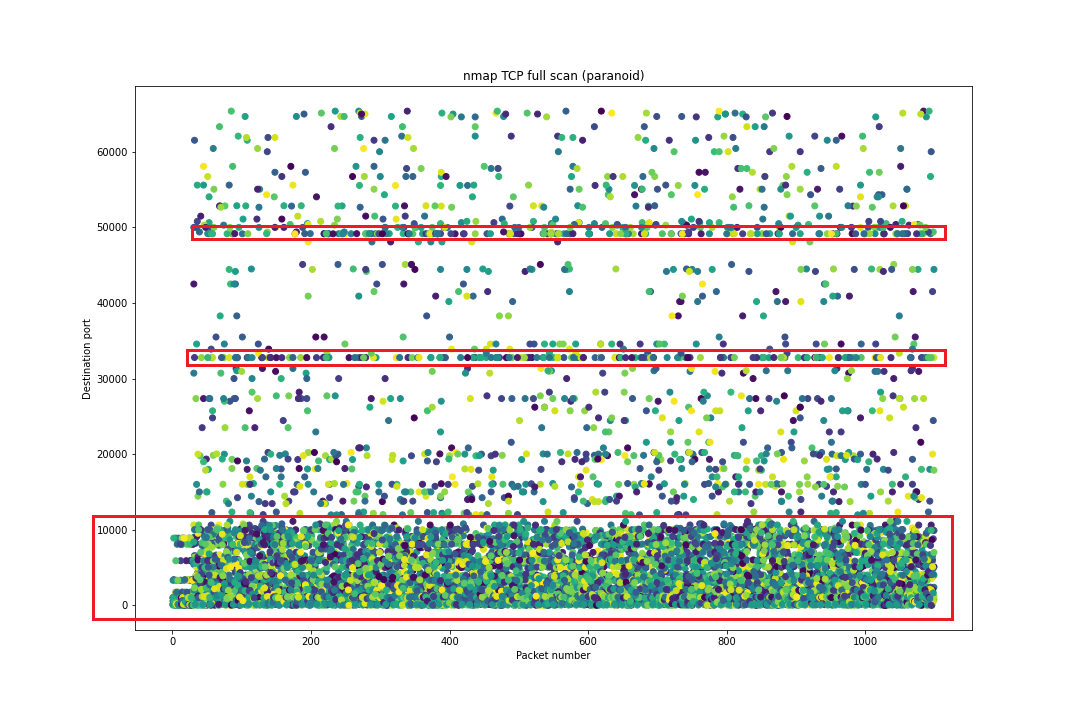
\includegraphics[width=8.2cm]{images/analysis/tcpsynscan/paranoid/DstPacketNrMarked.png} }
    \caption{Destination port sequence with various scan types and timing templates}%
    \label{fig:DstPortSequenceMisc}%
\end{figure}
\vfill
\clearpage

\newpage
\vfill


In figure \ref{fig:DstPortSequenceMisc} similarities are highlighted.
By further looking at these patterns, the same patterns can be seen in figure \ref{fig:DstIPIDSequenceMisc} only with a flipped x and y-axis.
Though within figure \ref{fig:DstIPIDSequenceMisc} the values of the IP ID field is used instead of the packet number as seen in figure \ref{fig:DstPortSequenceMisc}.
It is clear from the figure that the values of the IP ID field go through the whole specter close to 0 up to over 60000.
Adding one line of code at the end of the Jupyter notebook for printing the $ip\_ids$ variable, which is a list, confirms this.
This line was added to the $nmap\_null\_scan\_polite$ notebook, and the result from this shows the lowest IP ID field to be $13$, while the highest was $65533$.

\begin{figure}[!ht]%
    \centering
    \subfloat[fin scan insane\label{fig:FinInsDstIPID}]{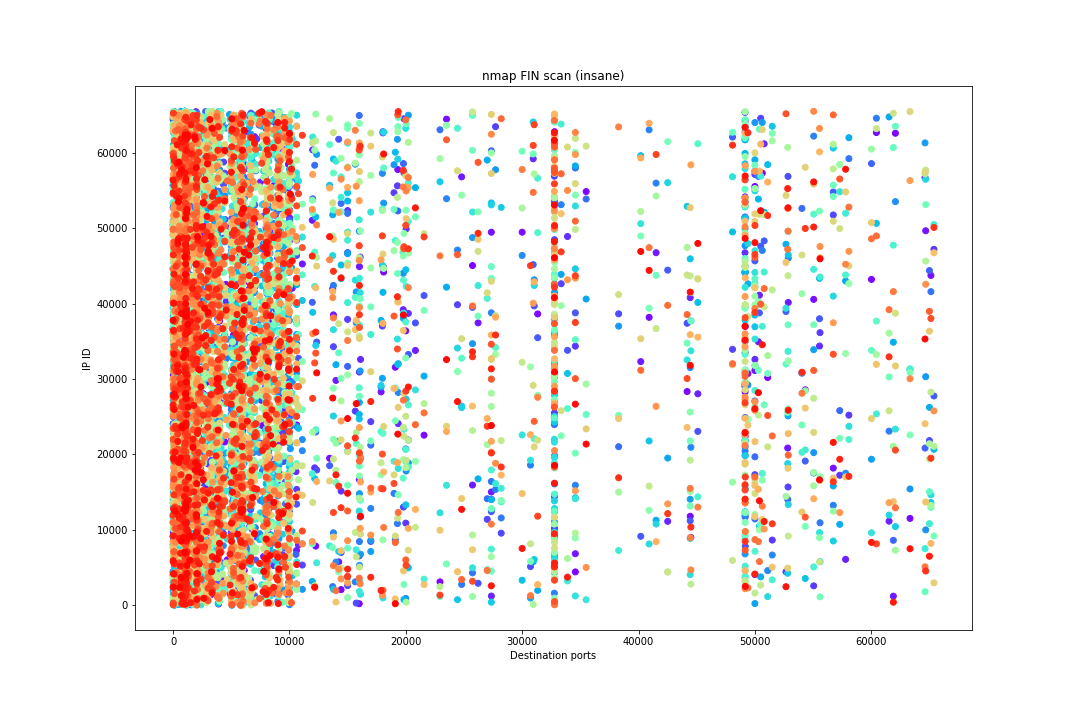
\includegraphics[width=8.2cm]{images/analysis/finscan/insane/IPIDDstPort.png} }
    \subfloat[ping scan aggressive\label{fig:PngAgrDstIPID}]{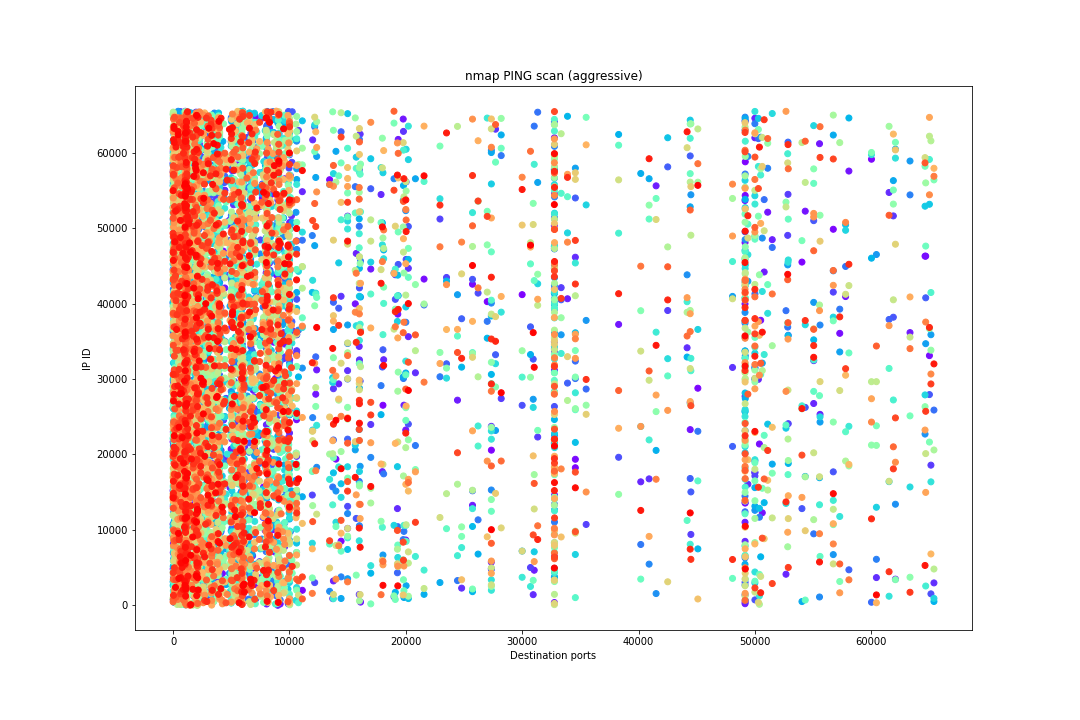
\includegraphics[width=8.2cm]{images/analysis/pingscan/aggressive/IPIDDstPort.png} } \\
    \subfloat[service discovery normal\label{fig:SvcNorDstIPID}]{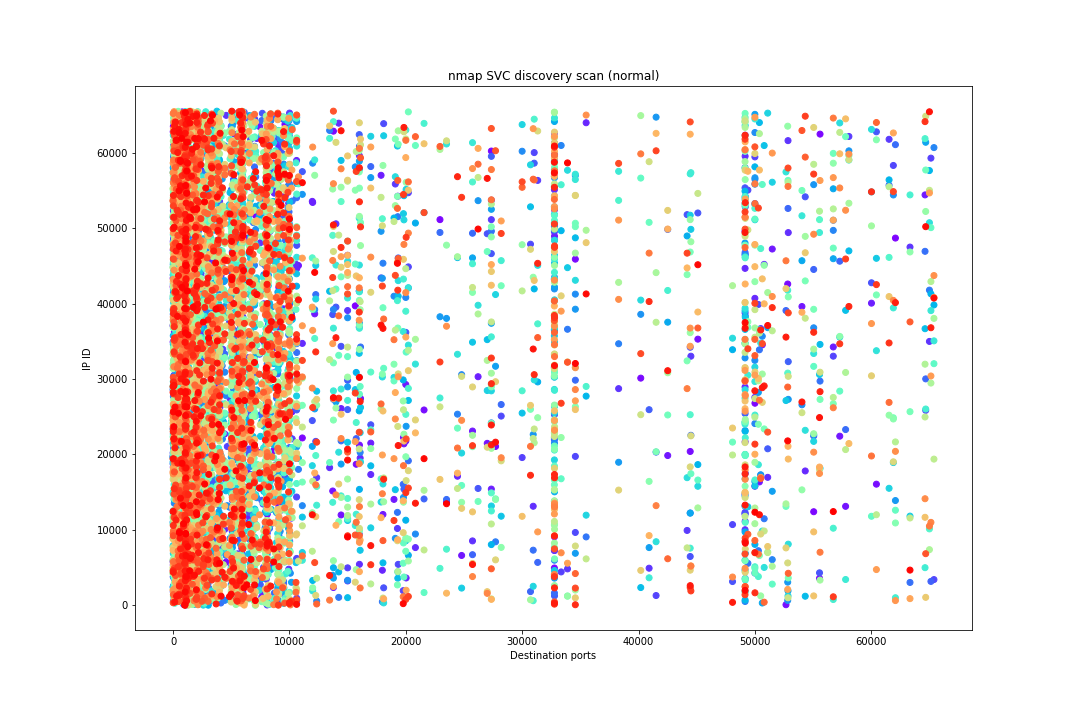
\includegraphics[width=8.2cm]{images/analysis/svcscan/normal/IPIDDstPort.png} }
    \subfloat[null scan polite\label{fig:NullPolDstIPID}]{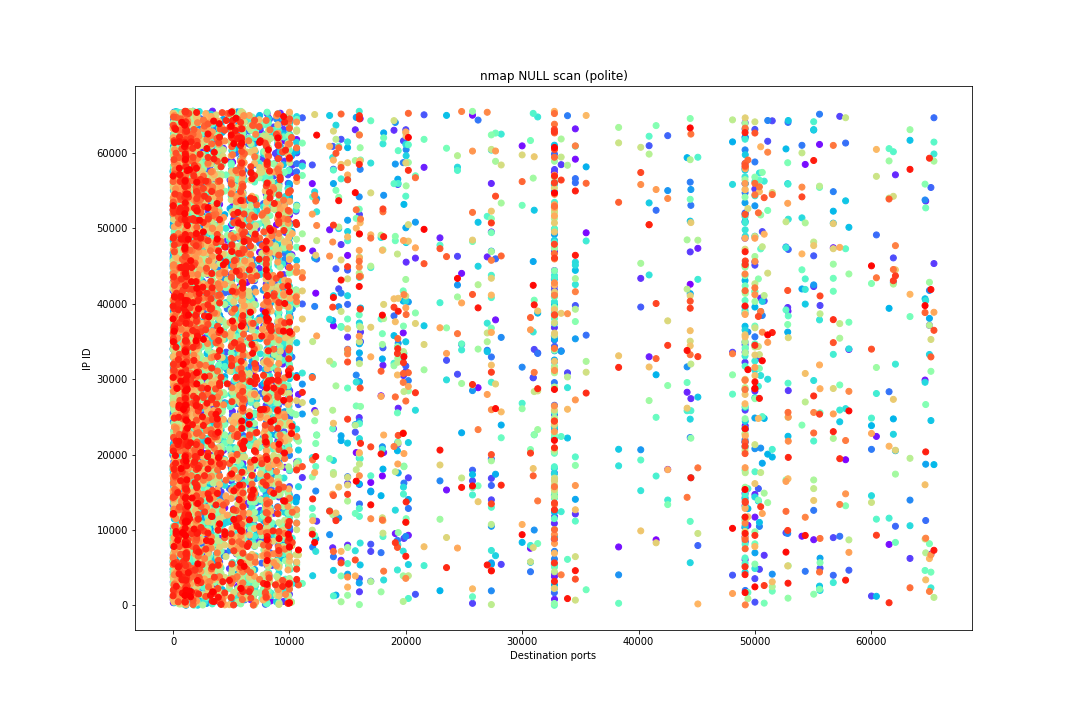
\includegraphics[width=8.2cm]{images/analysis/nullscan/polite/IPIDDstPort.png} } \\
    \subfloat[xmas scan sneaky\label{fig:XmasSneDstIPID}]{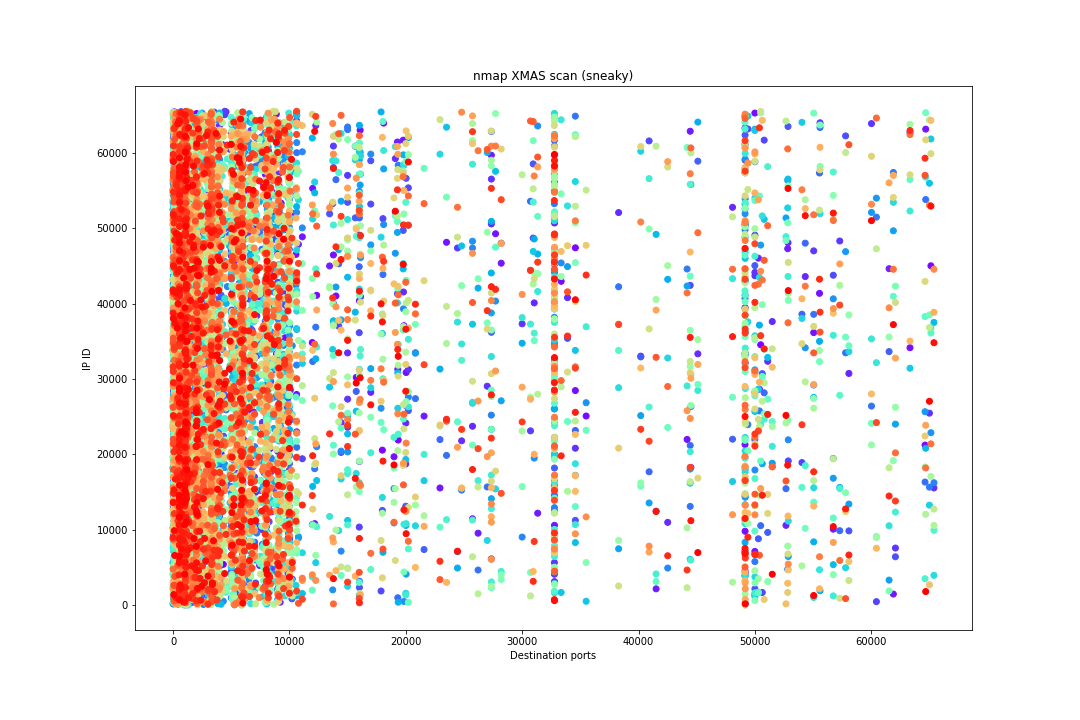
\includegraphics[width=8.2cm]{images/analysis/xmasscan/sneaky/IPIDDstPort.png} }
    \subfloat[TCP SYN paranoid\label{fig:TcpParDstIPID}]{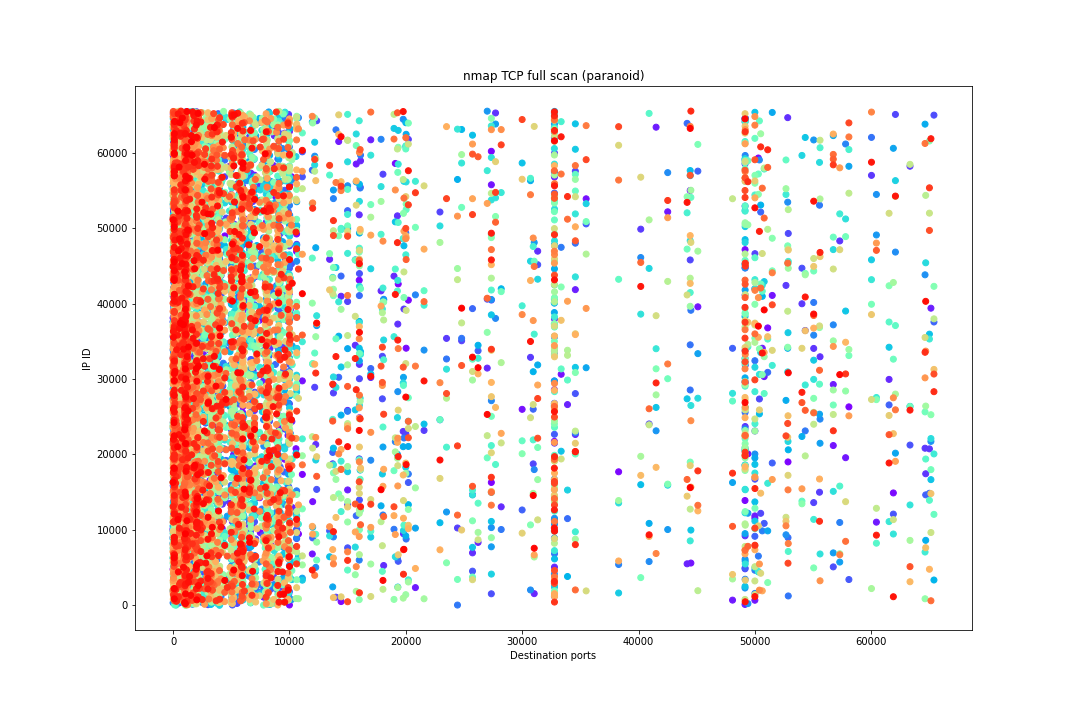
\includegraphics[width=8.2cm]{images/analysis/tcpsynscan/paranoid/IPIDDstPort.png} }
    \caption{Destination port and IP ID with various scan types and timing templates}%
    \label{fig:DstIPIDSequenceMisc}%
\end{figure}

Further in the analysis, the IP ID correlated with the destination port, shown in figure \ref{fig:DstIPIDSequenceMisc}, in a diagram shows the similar plots as in the port sequence diagram in figure \ref{fig:DstPortSequenceMisc}. The main part of ports targeted are under or close to 10000, and there's a line above 30000 and a new line just below 50000.
By rotating the diagram in figure \ref{fig:DstIPIDSequenceMisc} 90 degrees to the left, these plots could be compared to figure \ref{fig:ScanNumberDstPort} which clearly shows the same patterns as the destination port is a common denominator between the two mentioned figures.
